\section{Presentazione dello stage}
	\subsection{}
		\begin{frame}{ERA - Enterprise Remote Assistance}
			\begin{minipage}{\textwidth}
				\begin{minipage}{0.60\textwidth}
					\begin{itemize}
						\item Ricevere istruzioni sulle attività da svolgere
						\item Eseguire passaggi e procedimenti operativi
						\item Condividere informazioni
						\item Offrire supporto in tempo reale
					\end{itemize}
				\end{minipage}
				\begin{minipage}{0.30\textwidth}
					\begin{figure}
						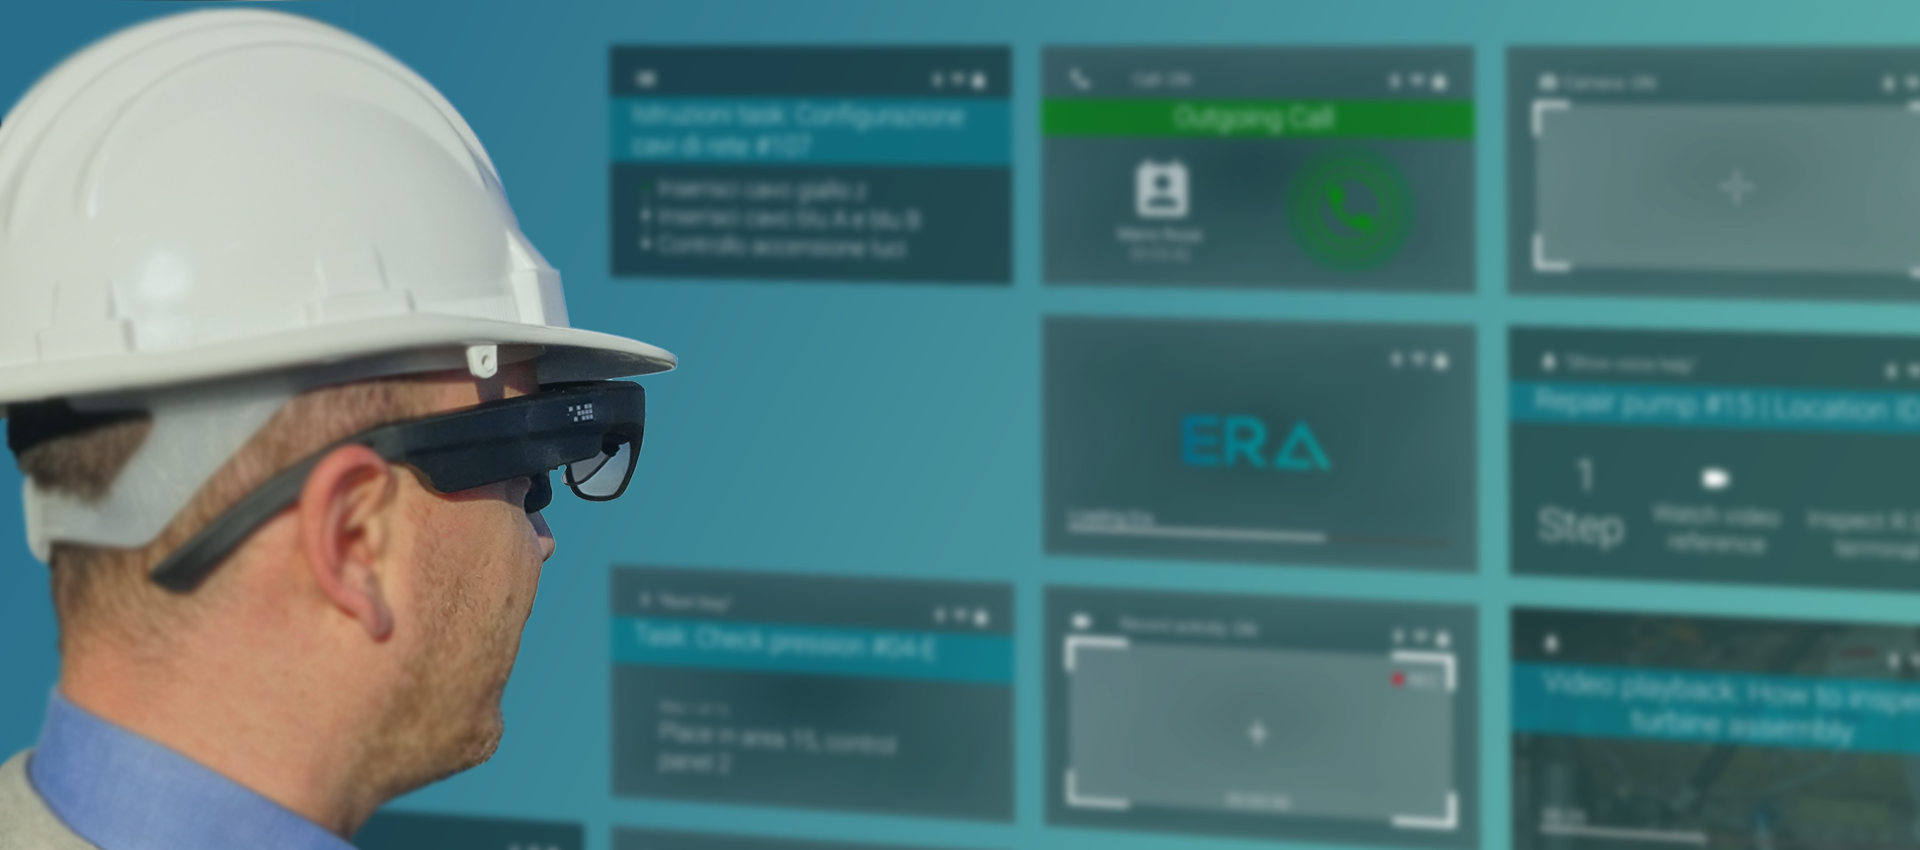
\includegraphics[width=1.5\textwidth]{capitolo_2/immagini/era.png}
					\end{figure}
				\end{minipage}
			\end{minipage}
		\end{frame}
	\subsection{}
		\begin{frame}{Tecnologie}
			\begin{center}
				\begin{minipage}{\textwidth}
					\begin{minipage}{0.29\textwidth}
						
\includegraphics[width=0.5\textwidth]{capitolo_2/immagini/java.png}
					\end{minipage}
					\begin{minipage}{0.60\textwidth}
						\begin{block}{\emph{Server Java}}
							\begin{itemize}
								\item Creazione e gestione canale di comunicazione
								\item Gestione utenti
								\item Sistema di autenticazione
							\end{itemize}
						\end{block}
					\end{minipage}
				\end{minipage}
				\vspace{2mm}
				\begin{minipage}{\textwidth}
					\begin{minipage}{0.60\textwidth}
						\begin{block}{\emph{Applicazione Android}}
							\begin{itemize}
								\item Prototipo lato \emph{client}
								\item Chat
								\item \emph{Streaming} audio-video
							\end{itemize}
						\end{block}
					\end{minipage}
					\begin{minipage}{0.29\textwidth}
							\begin{flushright}
								
\includegraphics[width=0.9\textwidth]{capitolo_2/immagini/android.png}
							\end{flushright}
					\end{minipage}
				\end{minipage}
			\end{center}
		\end{frame}
